\documentclass[aspectratio=169,10pt]{beamer}
\usepackage{amsmath,amssymb,booktabs,graphicx,array}
\usefonttheme{professionalfonts}
\setbeamertemplate{navigation symbols}{}
\setbeamertemplate{footline}{%
  \raisebox{10pt}{\makebox[\paperwidth]{\hfill\makebox[7em]{\normalsize\texttt{\insertframenumber/\inserttotalframenumber}}}}%
}
\newcommand{\src}[1]{\vfill{\tiny\color{gray}Source: \texttt{\detokenize{#1}}}}
\begin{document}

\section{Data}
\begin{frame}{Data | CRSP Daily, 2024-01-02 to 2024-12-31}
\small Actual rows at the beginning and end of the sample; one row is one security-day.\par\vspace{.5em}
\begin{center}\scriptsize\renewcommand{\arraystretch}{1.08}
\begin{tabular}{rrrrrrr}
\toprule
date & PERMNO & openprc & prc & vol & ret & shrout \\
\midrule
01-02 & 10026 & 165.97 & 168.86 & 89,969 & 0.010291 & 19,367 \\
01-02 & 10028 & 4.88 & 4.71 & 18,599 & -0.030864 & 26,700 \\
01-02 & 10032 & 106.36 & 106.35 & 78,780 & -0.016462 & 27,504 \\
01-02 & 10044 & 4.69 & 4.94 & 7,736 & 0.073913 & 6,304 \\
01-02 & 10065 & 17.60 & 17.45 & 235,208 & -0.014681 & 120,810 \\
01-02 & 10066 & 3.39 & 3.35 & 32,753 & -0.011800 & 11,784 \\
\midrule
12-31 & 10026 & 156.23 & 155.13 & 52,207 & -0.001095 & 19,478 \\
12-31 & 10028 & 7.22 & 7.18 & 9,659 & -0.001391 & 25,996 \\
12-31 & 10032 & 157.50 & 156.48 & 101,562 & -0.001340 & 27,092 \\
12-31 & 10044 & 2.40 & 2.43 & 10,438 & -0.004098 & 7,598 \\
12-31 & 10065 & 20.36 & 20.20 & 219,627 & -0.004926 & 112,690 \\
12-31 & 10066 & 4.88 & 4.90 & 24,310 & 0.006160 & 11,784 \\
\bottomrule
\end{tabular}\end{center}
\src{data/crsp_dsf_2024.csv.gz}
\end{frame}

\begin{frame}{Data | Point-in-time filter build}
\begin{center}\large\renewcommand{\arraystretch}{1.3}
\begin{tabular}{p{7.0cm}r}
\toprule
Security-day stage & Rows \\
\midrule
Raw CRSP Daily & 2,400,962 \\
Effective-date name match & 2,400,962 \\
Common shares and main exchanges & 987,277 \\
Signal-day $|\mathrm{prc}|\geq\$5$ & 702,841 \\
Complete features and available label horizon & 633,995 \\
\bottomrule
\end{tabular}\end{center}\par
\vspace{.4em}
\small $\mathrm{SHRCD}\in\{10,11\}$ and $\mathrm{EXCHCD}\in\{1,2,3\}$ are evaluated on each signal date. Raw file: 252 trading days and 10,503 PERMNOs.
\src{data_audit.csv; run_metadata.json}
\end{frame}

\begin{frame}{Data | Check the meanings and units}
\begin{columns}[T]
\begin{column}{.5\textwidth}
\begin{block}{RET is a holding-period return}
For PERMNO 10026 on Jan 2, $\mathrm{openprc}=165.97$, $\mathrm{prc}=168.86$, and $\mathrm{ret}=0.010291$.
\[168.86/165.97-1=0.01741\ne 0.010291.\]
The open-to-close price change is a different quantity.
\end{block}
\end{column}
\begin{column}{.46\textwidth}
\begin{block}{Units used in features}
\[\mathrm{shares}=1000\,\mathrm{shrout}\]
\[\mathrm{market\ cap}=|\mathrm{prc}|\times\mathrm{shares}\]
CRSP negative \texttt{prc} marks a bid/ask average; $|\mathrm{prc}|$ supplies price magnitude.
\end{block}
\end{column}
\end{columns}
\src{data/crsp_dsf_2024.csv.gz; WRDS CRSP data definitions}
\end{frame}

\begin{frame}{Data | Eight predictors from the trailing 20 market days}
\small Let $W_t$ be the 20-market-day window ending at signal close $t$. Each statistic requires at least 10 observations.\par\vspace{.3em}
\begin{center}\scriptsize\renewcommand{\arraystretch}{1.14}
\begin{tabular}{lp{7.3cm}}
\toprule
Feature & Definition on $W_t$ \\
\midrule
Trading days & Count of valid-price observations \\
Median price & Median $|\mathrm{prc}|$ \\
ADV & Mean share volume \\
Median dollar volume & Median $|\mathrm{prc}|\times\mathrm{vol}$ \\
ADV dollar & Mean $|\mathrm{prc}|\times\mathrm{vol}$ \\
Median turnover & Median $\mathrm{vol}/(1000\,\mathrm{shrout})$ \\
Annualized volatility & $\sqrt{252}\,\operatorname{sd}(\mathrm{ret})$ \\
Median market cap & Median $|\mathrm{prc}|\times1000\,\mathrm{shrout}$ \\
\bottomrule
\end{tabular}\end{center}
\src{src/run_crsp_benchmark_2024.py}
\end{frame}

\begin{frame}{Data | Response and executable timing}
\small $i$ denotes PERMNO and $t$ denotes a market day. $X_{i,t}\in\mathbb R^8$ is known after close $t$.\par\vspace{.4em}
\begin{center}
\fbox{Signal after close $t$}\quad$\longrightarrow$\quad\fbox{Fill at close $t+1$}\quad$\longrightarrow$\quad\fbox{Exit at close $t+2$}
\end{center}
\vspace{.5em}
\begin{block}{Primary response: realized holding-period return}
\[Y_{i,t}=R_{i,(t+1,t+2]}=\begin{cases}(1+r)(1+r^{DL})-1,&r,r^{DL}\text{ both observed},\\ r\text{ or }r^{DL},&\text{only one observed.}\end{cases}\]
\end{block}
\small Auxiliary direction label: $Z_{i,t}=\mathbf1\{Y_{i,t}>0\}$. No label is formed if the entry cannot fill or both return fields are missing.
\src{doc/pipeline.md; src/run_crsp_benchmark_2024.py}
\end{frame}

\section{Problem}
\begin{frame}{Problem | Estimate return and daily cross-sectional rank}
\begin{block}{Prediction in fold $k$ with model $m$}
\[\widehat Y_{i,t}^{(m,k)}=f_{m,k}(X_{i,t}),\qquad
f_{m,k}:\mathbb R^8\longrightarrow\mathbb R.\]
\end{block}
\small $f_{m,k}$ is fitted using only the fold's training and validation data; $\widehat Y$ is its return forecast.\par\vspace{.3em}
\[\mathrm{MSE}_m=\frac{1}{N}\sum_{i,t}(Y_{i,t}-\widehat Y_{i,t}^{(m,k)})^2,\qquad
\mathrm{RankIC}_{m,t}=\rho_{\mathrm S}\!\left(\widehat Y_{\cdot,t}^{(m,k)},Y_{\cdot,t}\right).\]
\small $\rho_{\mathrm S}$ is Spearman correlation among stocks observed on day $t$. Secondary test: estimate $P(Z_{i,t}=1\mid X_{i,t})$. Economic test: rank-based long--short return after costs.
\src{doc/pipeline.md; src/run_crsp_monthly_walkforward_2024.py}
\end{frame}

\section{Approach}
\begin{frame}{Approach | Daily observations, monthly walk-forward}
\begin{center}\scriptsize\renewcommand{\arraystretch}{1.13}
\begin{tabular}{llllrrr}
\toprule
Test block & Train through & Validate & Test dates & Train rows & Val. rows & Test rows \\
\midrule
July & May 29 & Jun 3--26 & Jul 1--31 & 233,220 & 46,591 & 60,347 \\
August & Jun 26 & Jul 1--29 & Aug 1--30 & 285,313 & 54,804 & 59,828 \\
September & Jul 29 & Aug 1--28 & Sep 3--30 & 345,555 & 54,349 & 54,400 \\
October & Aug 28 & Sep 3--26 & Oct 1--31 & 405,407 & 48,927 & 62,431 \\
November & Sep 26 & Oct 1--29 & Nov 1--26 & 459,792 & 56,950 & 49,040 \\
\bottomrule
\end{tabular}\end{center}
\vspace{.5em}
\begin{center}\fbox{Expanding train}\quad$\longrightarrow$\quad\fbox{Prior-month validation}\quad$\longrightarrow$\quad\fbox{Daily test forecasts}\end{center}
\small Two-market-day label gap at each boundary; December outcomes stay sealed.
\src{run_metadata.json}
\end{frame}

\begin{frame}{Approach | Fixed baselines and fitted models}
\small\renewcommand{\arraystretch}{1.2}
\begin{tabular}{p{2.1cm}p{8.1cm}}
\toprule
Model & Forecast or fitting rule \\
\midrule
Zero & $\widehat Y=0$; MSE reference \\
Reversal & $\widehat Y=-\mathrm{ret}_{i,t}$; fixed one-day reversal score \\
Ridge & $\min_{\beta}\|Y-X\beta\|_2^2+\alpha\|\beta\|_2^2$; $\alpha\in\{0.1,10,1000\}$ \\
Boosted tree & Histogram gradient boosting; 80 rounds, learning rate 0.05, leaves $\in\{3,7\}$ \\
Logistic & $P(Z=1\mid X)=\sigma(\beta_0+X^\top\beta)$; $C=1$ \\
\bottomrule
\end{tabular}\par
\vspace{.65em}
\small Ridge and tree settings minimize prior-month validation MSE. Final regression fit uses train $+$ validation; median imputation and scaling are fitted within each fold.
\src{src/run_crsp_monthly_walkforward_2024.py}
\end{frame}

\begin{frame}{Approach | Rank portfolio and cost equation}
\small On each signal day, select top and bottom predicted-return deciles; $L_t$ and $S_t$ are the selected sets.\par
\[w_{i,t}=\begin{cases}+1/|L_t|,&i\in L_t,\\-1/|S_t|,&i\in S_t,\\0,&\text{otherwise.}\end{cases}\]
\vspace{-.3em}
\[r_t^{\rm gross}=\sum_i w_{i,t}Y_{i,t},\qquad
\mathrm{TO}_t=\sum_i|w_{i,t}-w_{i,t-1}|,\qquad
r_t^{\rm net}=r_t^{\rm gross}-\underbrace{10^{-3}}_{\text{10 bps per turnover unit}}\mathrm{TO}_t.\]
\small Both sides are equal weight. A portfolio date is scored only if every selected holding has an observed outcome.
\src{src/run_crsp_benchmark_2024.py; run_metadata.json}
\end{frame}

\section{Result}
\begin{frame}{Result | Prediction gains across 105 daily tests}
\begin{center}\begin{tabular}{lrrr}
\toprule
Model & Test MSE & Mean IC & Mean Rank IC \\
\midrule
Zero & 0.00131959 & --- & --- \\
Reversal & 0.00267757 & 0.00316 & 0.00590 \\
Ridge & 0.00131761 & 0.00666 & 0.01104 \\
Boosted tree & \textbf{0.00131746} & \textbf{0.01364} & \textbf{0.01276} \\
\bottomrule
\end{tabular}\end{center}
\vspace{.55em}
\small 285,882 of 286,046 daily test predictions have valid labels. The tree leads in Rank IC; its MSE gain relative to zero is about 0.16\%.
\src{model_comparison.csv; predictions.csv.gz}
\end{frame}

\begin{frame}{Result | Daily cross-sectional Rank IC}
\begin{center}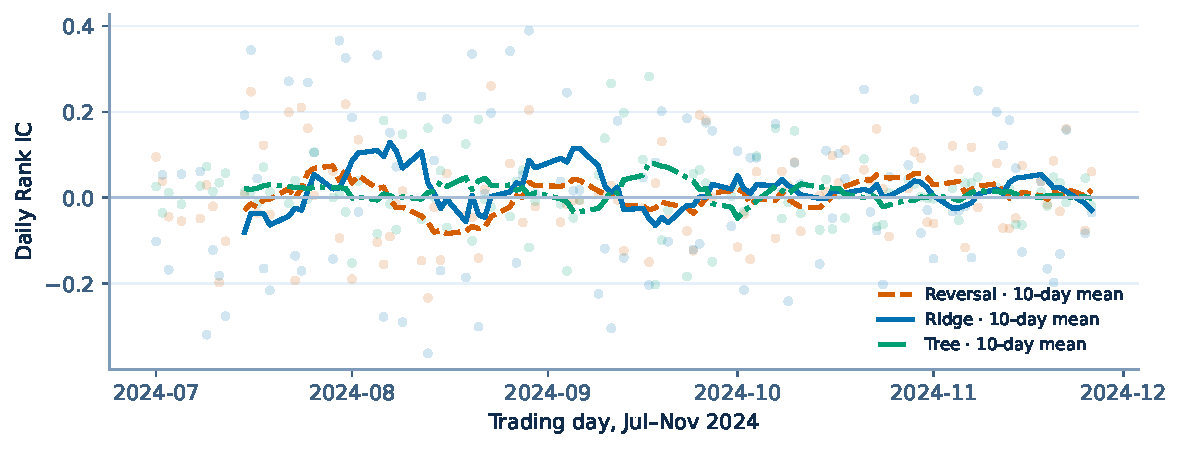
\includegraphics[width=.82\textwidth]{figures/daily_rank_ic.pdf}\end{center}
\small Dots represent individual trading days; lines are 10-day rolling means. Color and line pattern distinguish reversal, Ridge, and tree.
\src{ic_reversal.csv; ic_ridge.csv; ic_tree.csv}
\end{frame}

\begin{frame}{Result | Net portfolio return on observed days}
\begin{center}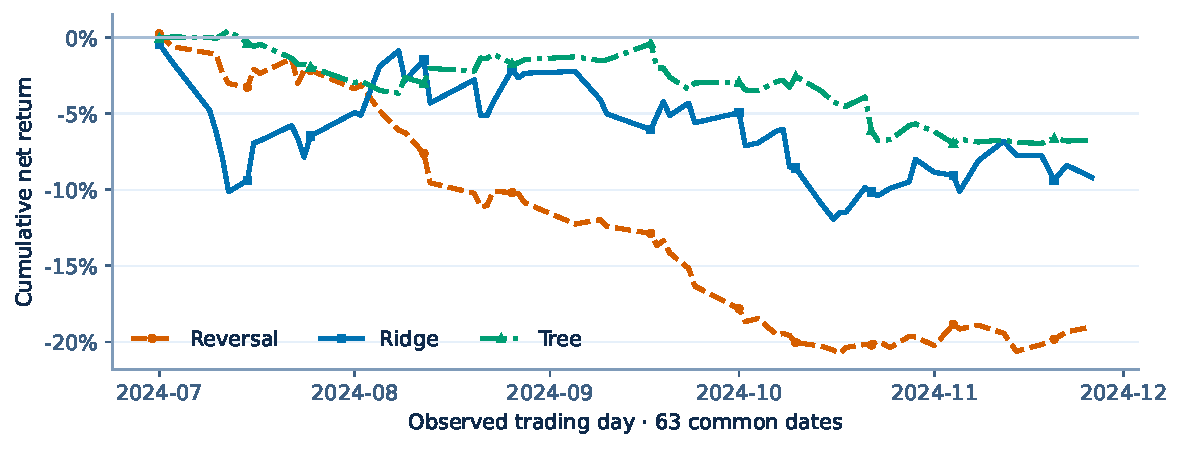
\includegraphics[width=.82\textwidth]{figures/net_portfolio_common.pdf}\end{center}
\small Cumulative net return uses 63 dates with complete selected-holding outcomes for all three strategies. It is a conditional comparison.
\src{portfolio_reversal.csv; portfolio_ridge.csv; portfolio_tree.csv}
\end{frame}

\begin{frame}{Result | Trading costs and direction classification}
\begin{columns}[T]
\begin{column}{.51\textwidth}
\small\begin{tabular}{lrr}
\toprule
Portfolio & Net Sharpe & Mean turnover \\
\midrule
Reversal & -6.350 & 3.31 \\
Ridge & -1.527 & 0.33 \\
Boosted tree & -2.852 & 0.20 \\
\bottomrule
\end{tabular}
\end{column}
\begin{column}{.44\textwidth}
\begin{block}{Logistic classifier}
\small ROC-AUC: 0.5032\\Balanced accuracy: 50.41\%\\Cross-entropy: 0.69293
\end{block}
\end{column}
\end{columns}
\vspace{.5em}
\small Sharpe uses 63 common dates at 10 bps per turnover unit. Selected-holding outcomes are incomplete on 15, 36, and 21 of the 105 test days for reversal, Ridge, and tree.
\src{model_comparison.csv; classification_metrics.csv}
\end{frame}

\section{Conclusion}
\begin{frame}{Conclusion | Small ranking signal, limited trading evidence}
\begin{enumerate}
\item Boosted tree has the highest stitched Rank IC (0.0128), a small edge over Ridge (0.0110).
\item Direction classification is near chance (AUC 0.5032).
\item All three portfolios have negative net Sharpe on the 63 comparable dates under the stated cost.
\item Missing selected-holding outcomes limit inference about the complete 105-day portfolio path.
\end{enumerate}
\vspace{.5em}
\begin{block}{Next step}
Resolve missing exit returns, then rerun the same daily portfolio protocol on a complete set of test dates.
\end{block}
\src{model_comparison.csv; classification_metrics.csv; run_metadata.json}
\end{frame}
\end{document}
